\documentclass[12pt,a4paper]{report}
\usepackage[utf8]{inputenc}
\usepackage{geometry}
\usepackage{setspace}
\usepackage{titlesec}
\usepackage{graphicx}
\usepackage{subcaption}
\usepackage{amsmath}
\usepackage{hyperref}
\usepackage{ragged2e}
\usepackage{lmodern}
\usepackage{array}

% Page setup
\geometry{margin=1in}
\onehalfspacing
\setlength{\parindent}{1.5em} 
\setlength{\parskip}{0.5em}


% Chapter formatting
\titleformat{\chapter}[display]
  {\bfseries\Large}
  {\filleft\Huge\thechapter}
  {1ex}
  {\titlerule\vspace{1ex}\filright}


% Hyperlink setup
\hypersetup{
    colorlinks=true,
    linkcolor=blue,
    urlcolor=blue,
    citecolor=blue
}


\begin{document}
% Title Page
\begin{titlepage}
    \begin{center}
        \large\textbf{GEOPHYSISCAL EVALUATION OF SUBSURFACE LAYERS FOR CIVIL}
        \large\textbf{ENGINEERING FOUNDATION USING ELECTRICAL RESISTIVITY METHODS} \\[3.3cm]
        
        By: \\[0.2cm]
        
        \Large\textbf{SURAJUDEEN HADI ADEMOLA} \\[0.1cm]
        \Large\textbf{B.Sc Physics (U.I)} \\[0.1cm]
        \Large\textbf{222814} \\[3.3cm]
        
        \large\textbf{A PROJECT SUBMITTED TO THE DEPARTMENT OF PHYSICS FACULTY OF SCIENCE
        UNIVERSITY OF IBADAN IN IMPARTIAL FULFILMENT FOR THE AWARD OF BACHELOR IN SCIENCE (B.Sc) \\
        DEGREE IN PHYSICS/SOLID EARTH PHYSICS} \\[4cm]
        
        \textbf{JANUARY, 2025}
    \end{center}
\end{titlepage}

\pagenumbering{roman}

% Dedication
\chapter*{Dedication}
\addcontentsline{toc}{chapter}{Dedication} 
\justifying
This will be provided later

% Acknowledgements
\chapter*{Acknowledgements}
\addcontentsline{toc}{chapter}{Acknowledgements}
\justifying
This will be provided

% Abstract
\chapter*{Abstract}
\addcontentsline{toc}{chapter}{Abstract} 
\justifying
This will be provided later

% List of Figures
\listoffigures
\addcontentsline{toc}{chapter}{List of Figures}

% List of Tables
\listoftables
\addcontentsline{toc}{chapter}{List of Tables}

% Table of Contents
\tableofcontents

% Certification
\chapter*{Certification}
\addcontentsline{toc}{chapter}{Certification} 
\justifying
This will be provided later

\newpage

\pagenumbering{arabic}

% Chapter 1: INTRODUCTION
\chapter{CHAPTER 1: INTRODUCTION}
\numberwithin{equation}{chapter}

\section{Background to the Study}

Building failures, a prevalent issue in various regions, often result from poor soil conditions, inadequate site investigations, and a lack of understanding of the underlying subsurface structure. \textbf{(Amadi, Eze, \textit{et al.,} 2012)} highlight that improper foundation designs and insufficient knowledge of the structural distribution of subsurface layers are leading contributors to such failures. Furthermore, \textbf{(Kværna and \textbf{Øygarden} 2006)} emphasized that soil instability, often caused by moisture fluctuations, plays a significant role in compromising the structural integrity of buildings. To mitigate these risks, comprehensive geophysical surveys are vital for analyzing the physical properties of the ground before construction.

Recent studies have expanded the scope of geophysical methods like Vertical Electrical Sounding (VES) and Constant Separation Traversing (CST) to include subsurface mapping, groundwater exploration, and geotechnical evaluations. \textbf{(Adetoyinbo, \textit{et al.,} 2023)}, in their work published in the \textit{International Journal of Scientific and Applied Research}, used VES and GIS to assess groundwater potential and subsurface characteristics in Idi-Ayunre, Ibadan. Their study identified significant geological features, such as fracture zones and aquifer units, revealing areas with low groundwater prospects. They demonstrated how the integration of geophysical data with GIS can enhance decision-making in resource management.

Similarly, \textbf{(Ogunseye, \textit{et al.,} 2022)}, in their work published in the \textit{Journal of Environmental Studies}, analyzed the geochemical properties of soils in Mokola, Ibadan, using soil samples and laboratory tests. Their findings highlighted the presence of heavy metal contamination, emphasizing its potential impact on groundwater quality and the importance of including geochemical assessments in subsurface investigations.

The application of Constant Separation Traversing (CST) has also gained significant attention for its role in evaluating lateral resistivity variations and detecting geological discontinuities. \textbf{(Anomohanran, \textit{et al.,} 2016)} applied CST to investigate lateral subsurface variations in the Niger Delta region, highlighting its effectiveness in detecting faults, fractures, and lithological boundaries that may compromise the stability of engineering foundations. Their findings demonstrated how CST complements VES by providing lateral profiling of resistivity, offering a more comprehensive understanding of subsurface conditions. Furthermore, \textbf{(Ismaila, \textit{et al.,} 2019)} used CST in combination with VES to assess subsurface layers for road construction projects in Ilorin, Nigeria. Their work revealed significant variations in soil composition and resistivity, emphasizing the need for lateral resistivity profiling in regions with heterogeneous geological settings.

Geophysical surveys, including VES and CST, are particularly significant in regions where soil heterogeneity poses risks to construction activities. For example, \textbf{(Agada, Ibuot, and Oseghale, \textit{et al.,} 2013)} investigated subsurface characteristics in an area prone to structural failures. Their findings revealed that geological discontinuities, such as fractures and dislocations, were primary contributors to differential settlements and structural disintegration. This underscores the importance of employing methods like VES and CST, which can delineate subsurface features with precision. Electrical resistivity surveys have emerged as a popular method in geotechnical investigations due to their high spatial resolution, cost-effectiveness, and non-destructive nature. This method measures the ability of subsurface materials to conduct electrical currents, enabling the identification of various layers, voids, fractures, and lithological features. As noted by \textbf{(Griffiths and Barker 1993)}, and corroborated by \textbf{(Soupisos, \textit{et al.,} 2006)}, these surveys provide critical data that can prevent construction failures by ensuring that foundation designs align with the physical and structural characteristics of the site.

Furthermore, \textbf{(Warner 2004)} and \textbf{(Ozeqin, \textit{et al.,} 2017)} emphasized that geophysical techniques are indispensable tools for assessing the bearing capacity of soils. These methods enable civil engineers to identify areas of concern, such as seepage zones and clayey substrata, which can cause excessive settlement and cracking in buildings. By incorporating such techniques into site investigations, construction projects can significantly reduce the risks associated with geotechnical failures.

In practical terms, electrical resistivity methods, including VES and CST, have been successfully applied in various engineering projects to identify and map subsurface structures. According to \textbf{(Lapenna, \textit{et al.,} 2005)}, these methods are invaluable for delineating depth variations, subsurface discontinuities, and lithological interfaces that may affect foundation stability. In addition to their technical benefits, they offer a cost-effective solution compared to traditional drilling methods, making them accessible for large-scale geotechnical investigations.

In summary, the integration of \textbf{Vertical Electrical Sounding (VES)} and \textbf{Constant Separation Traversing (CST)} represents an innovative approach to geotechnical site investigation by addressing challenges related to subsurface heterogeneity and providing insights into lateral and vertical variations, these methods mitigate risks of construction failure. This study employs these techniques to evaluate the geotechnical characteristics of the subsurface within the study area, contributing to safer and more sustainable civil engineering practices.

\section{Research Problem}
Inadequate knowledge of subsurface conditions remains a critical factor contributing to building failures, particularly in regions with complex and heterogeneous geological settings. Engineers often face challenges in accurately assessing subsurface characteristics, which leads to poorly designed foundations that are unable to prevent excessive settling, structural cracking, or outright collapse. Despite advancements in construction technology, many civil engineering projects still suffer from cost overruns and safety concerns stemming from improper site investigations.
While geophysical methods such as Vertical Electrical Sounding (VES) and Constant Separation Traversing (CST) have demonstrated significant potential in subsurface characterization, their application in civil engineering foundation designs remains underexplored. This gap in the integration of effective site investigation techniques results in a lack of precise and actionable data, which not only compromises structural stability but also incurs substantial economic and safety risks. By addressing this issue, the study aims to highlight how the use of advanced geophysical methods can bridge this gap, mitigate construction-related challenges, and enhance sustainable engineering practices. This research focuses on leveraging VES and CST to provide comprehensive subsurface information, ensuring improved construction outcomes and safer foundation designs.

\section{Aims and Objectives}

\subsection{Aims of the Study}
The aim of this project is to evaluate the subsurface layers for civil engineering foundation design by employing electrical resistivity methods, specifically Vertical Electrical Sounding (VES) with Schlumberger configuration and Constant Separation Traversing (CST) with Wenner configuration, aiming to provide actionable insights for foundation stability.


\subsection{Objectives of the Study}
The specific objectives of this study are to:
\begin{itemize}
    \item Map the subsurface layers and determine their resistivity values using VES and CST methods.
    \item Identify weak zones, fractures, and groundwater presence that may affect the stability of civil engineering foundations.
    \item Analyze the depth, thickness, and resistivity of subsurface layers to assess their suitability for various foundation types.
    \item Detect lateral variations such as faults, fractures, or discontinuities using CST to complement the vertical subsurface evaluation.
    \item Correlate resistivity values with lithological and geotechnical properties, such as soil type, compaction, and strength.
    \item Combine VES and CST data to generate 3D visualization of the subsurface using specialized geophysical software, enhancing the interpretation and understanding of subsurface features.
    \item Provide engineering recommendations for foundation design based on geophysical findings, ensuring safety, cost-efficiency, and structural stability in the study area.
\end{itemize}

\section{Justification of the Study}
Understanding subsurface layers is essential for civil engineering foundation design, as inadequate knowledge can lead to structural failures, safety risks, and financial losses. The use of \textbf{Vertical Electrical Sounding (VES)} and \textbf{Constant Separation Traversing (CST)} offers a powerful, cost-effective, and non-invasive approach to addressing these challenges.

Previous studies, such as \textbf{Coker (2012)} in the Akobo area of Ibadan and \textbf{(Adagunodo, \textit{et al.} 2013)} in Oniye, Southwestern Nigeria, demonstrated the utility of VES for groundwater exploration and fracture detection. Similarly, research by \textbf{(Farinde, \textit{et al.} 2015)} focused on integrating geophysical and geotechnical methods for road construction at the University of Ibadan. However, these studies often emphasized resource exploration or general geotechnical characterizations rather than specifically addressing civil engineering foundation requirements.

Regions with heterogeneous soil conditions, like Ibadan, require tailored, localized geophysical evaluations to mitigate risks such as differential settlement, soil instability, and geological discontinuities. While earlier works provided valuable geological insights, there remains a significant gap in leveraging these findings for actionable recommendations in foundation design.

This study aims to fill this gap by explicitly integrating VES and CST methods to evaluate the lithological and structural characteristics of subsurface layers. VES will focus on vertical resistivity profiling, while CST will provide complementary lateral resistivity variations, making it possible to detect faults or fractures that could compromise foundation stability. By correlating resistivity data with geotechnical properties, this research delivers practical insights into soil properties, lithological variations, and structural integrity, enhancing the safety and cost-efficiency of construction practices.

Unlike previous studies, this research emphasizes civil engineering applications, offering a novel approach to geophysical evaluations tailored for foundation design. The findings will contribute to safe and sustainable construction practices, bridging the gap between geophysical insights and practical engineering solutions in complex geological settings.

\section{Geophysical Investigation}
In this research work, the geophysical survey was carried out using \textbf{Vertical Electrical Sounding (VES)} with the Schlumberger array electrode configuration and \textbf{Constant Separation Traversing (CST)} with the Wenner array electrode configuration. A total of \textbf{20 VES} profiles and \textbf{5 CST} profiles were conducted. The coordinates of the points in the selected area were taken, and the results were collated. The electrical resistivity method involves injecting current into the ground and measuring the resulting potential difference to determine subsurface resistivity variations. These variations help delineate different geological layers, assess lithological properties, and detect fractures or faults.

\section{Geological Settings}

\subsection{The Study Location}
Nigeria, located in West Africa, offers a rich and varied geological tapestry for geophysical research on subsurface layers, particularly for civil engineering foundations. The country's geology ranges from the ancient crystalline basement complex in the southwest, composed of migmatites, gneisses, and granites, to several significant sedimentary basins like the Niger Delta, the Benue Trough, and the Chad Basin. The basement complex's extensive weathering creates a regolith that significantly impacts foundation stability, necessitating thorough geophysical investigation to understand its depth and characteristics.

The sedimentary basins, especially the Niger Delta, present complex stratigraphy with layers of sand, silt, and clay, which have substantial implications for foundation design due to their variable thickness and composition. Hydrogeologically, Nigeria shows diversity with groundwater confined to fractured and weathered zones in the basement areas, contrasting with the broader aquifers in sedimentary regions, affecting soil moisture and stability. Structurally, the presence of faults, folds, and fractures across the nation dictates the subsurface's response to structural loads, crucial for avoiding issues like differential settlement. Even within these broad geological zones, local variability due to tectonic activity, erosion, and sediment deposition makes each site unique, particularly in areas like Ibadan where soil conditions can be highly heterogeneous.

Previous geophysical studies in Nigeria have laid a foundation for understanding how techniques like Vertical Electrical Sounding (VES) and Constant Separation Traversing (CST) can be applied to map and interpret these geological features for civil engineering purposes. This geological complexity and the existing research base make Nigeria an excellent location for advancing knowledge on how to ensure the safety and sustainability of civil engineering projects through geophysical evaluation of subsurface conditions. \\

\begin{figure}[h]
    \centering
    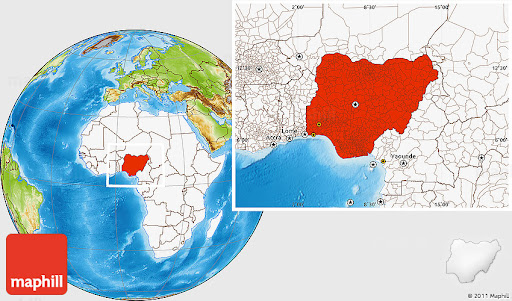
\includegraphics[width=1.0\textwidth]{map2.jpg}
    \caption{\textit{Map showing Nigeria from the World Map.}}
\end{figure}

\subsection{The Study Area}

The geophysical investigation for this study was conducted across two distinct locations within Ibadan North Local Governement at the University of Ibadan, Oyo State, Nigeria. This study area lies within the southwestern part of Nigeria, each chosen to represent different geological and soil conditions pertinent to civil engineering foundation design.

\subsubsection{\textbf{First Location:}}
Located at Emotan Lane near the University of Ibadan Central Mosque, Ibadan, with coordinates 7.44662° N, 3.89960° E, this site lies within the southwestern part of Nigeria. This area is characterized by the crystalline basement complex, typical of the region, with significant weathering that could impact foundation stability. Here, 10 Vertical Electrical Soundings (VES) were executed using the Schlumberger electrode configuration, and 3 Constant Separation Traversing (CST) profiles were conducted with the Wenner electrode configuration.

\subsubsection{\textbf{Second Location:}}
The second investigation site is at Appleton Road by Abubakar Abdulsalam Hall, University of Ibadan, with coordinates 7.43933° N, 3.89449° E. This location also represents the geological complexity of the area, featuring a mix of basement rocks with potential for varying soil compositions due to its proximity to different geological features. This site was chosen to assess how these conditions affect foundation stability and to understand the variability in soil composition. Here, 10 VES were similarly carried out, and 2 CST profiles were established.

Both areas were selected to provide a comprehensive understanding of the subsurface conditions within the University of Ibadan campus, ensuring the findings can be directly applicable to civil engineering practices in similar geological settings. The precise coordinates of these sites were meticulously recorded to enable accurate geophysical surveying and to facilitate future reference or validation of the study results.

\begin{figure}[!]
    \centering
    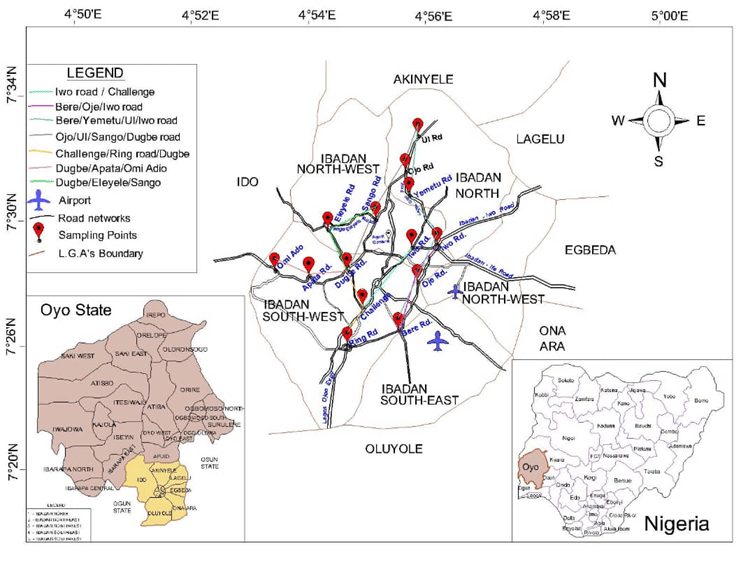
\includegraphics[width=1.0\textwidth]{Map-of-Ibadan-city.png}
    \caption{Map of Ibadan city in Oyo State, Nigeria showing the route.}
\end{figure}
\begin{figure}[!]
    \centering
        \centering
        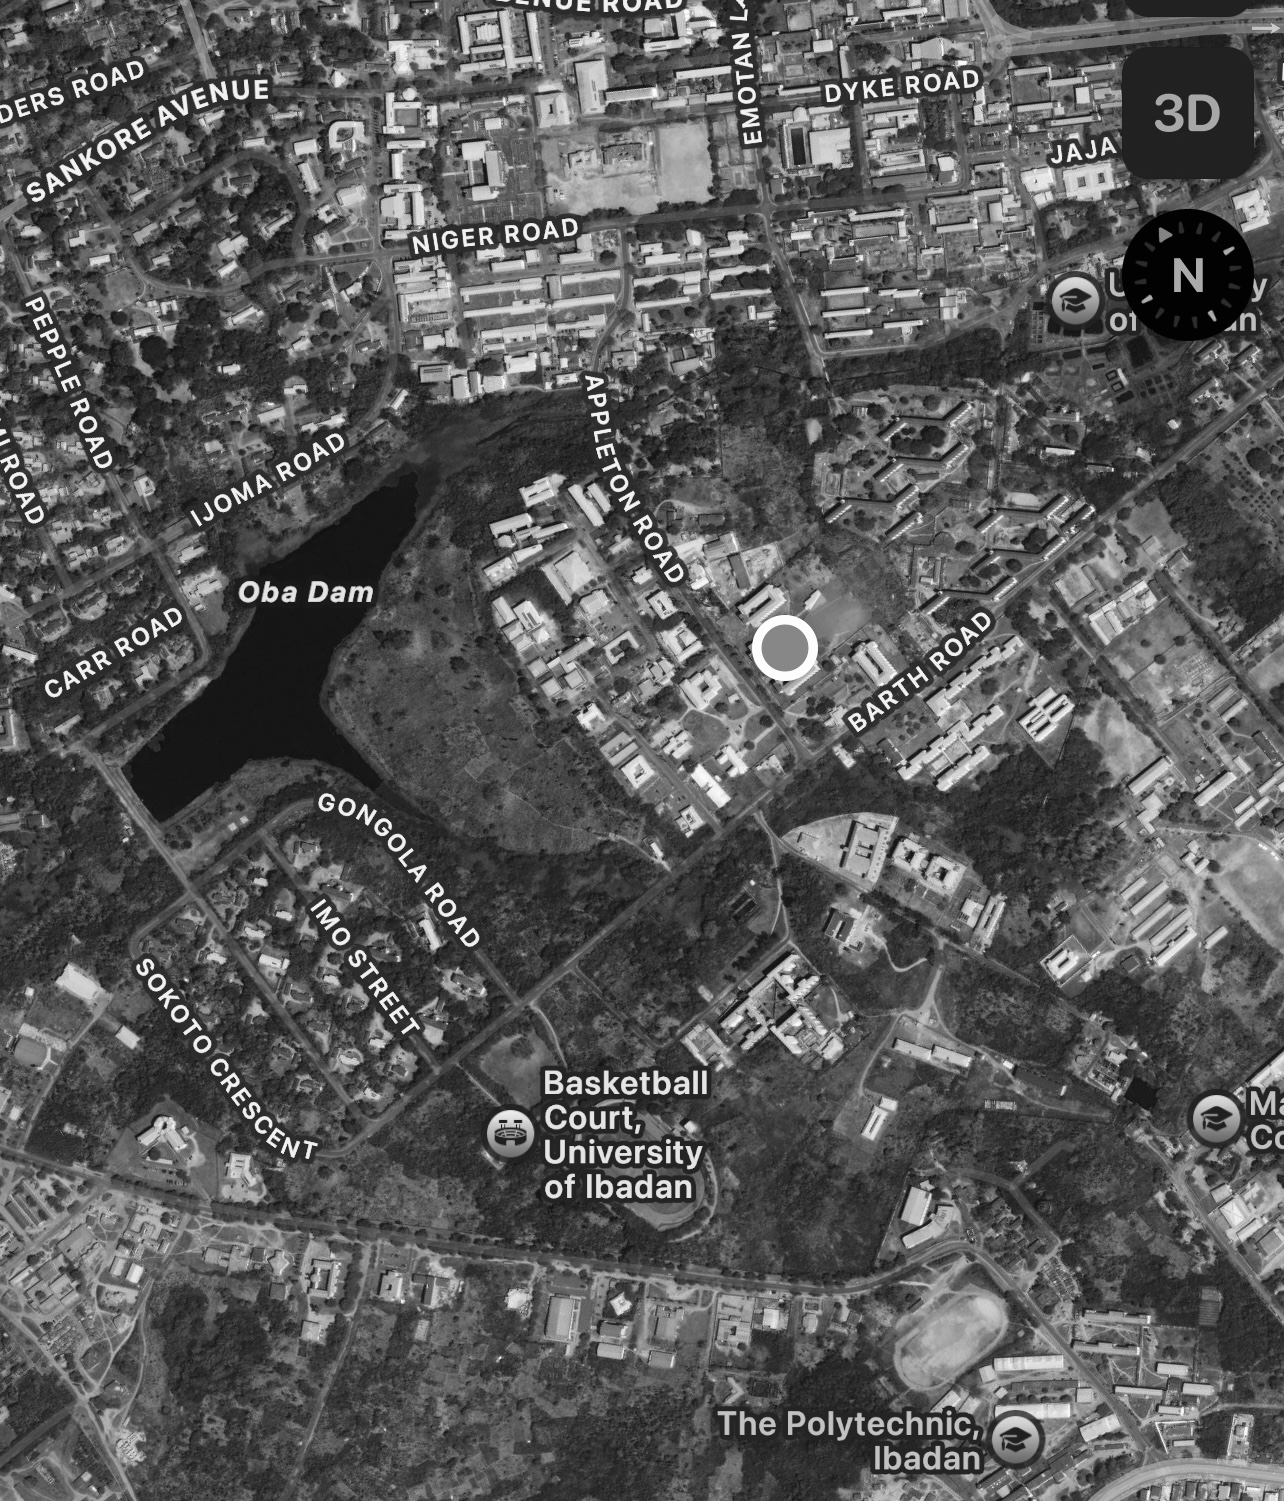
\includegraphics[width=1.0\textwidth]{MosqueMap.jpg}
        \caption{\textbf{Coordinates:} 7.44662° N, 3.89960° E.}
        \label{fig:first}
\end{figure}
\begin{figure}[!]
        \centering
        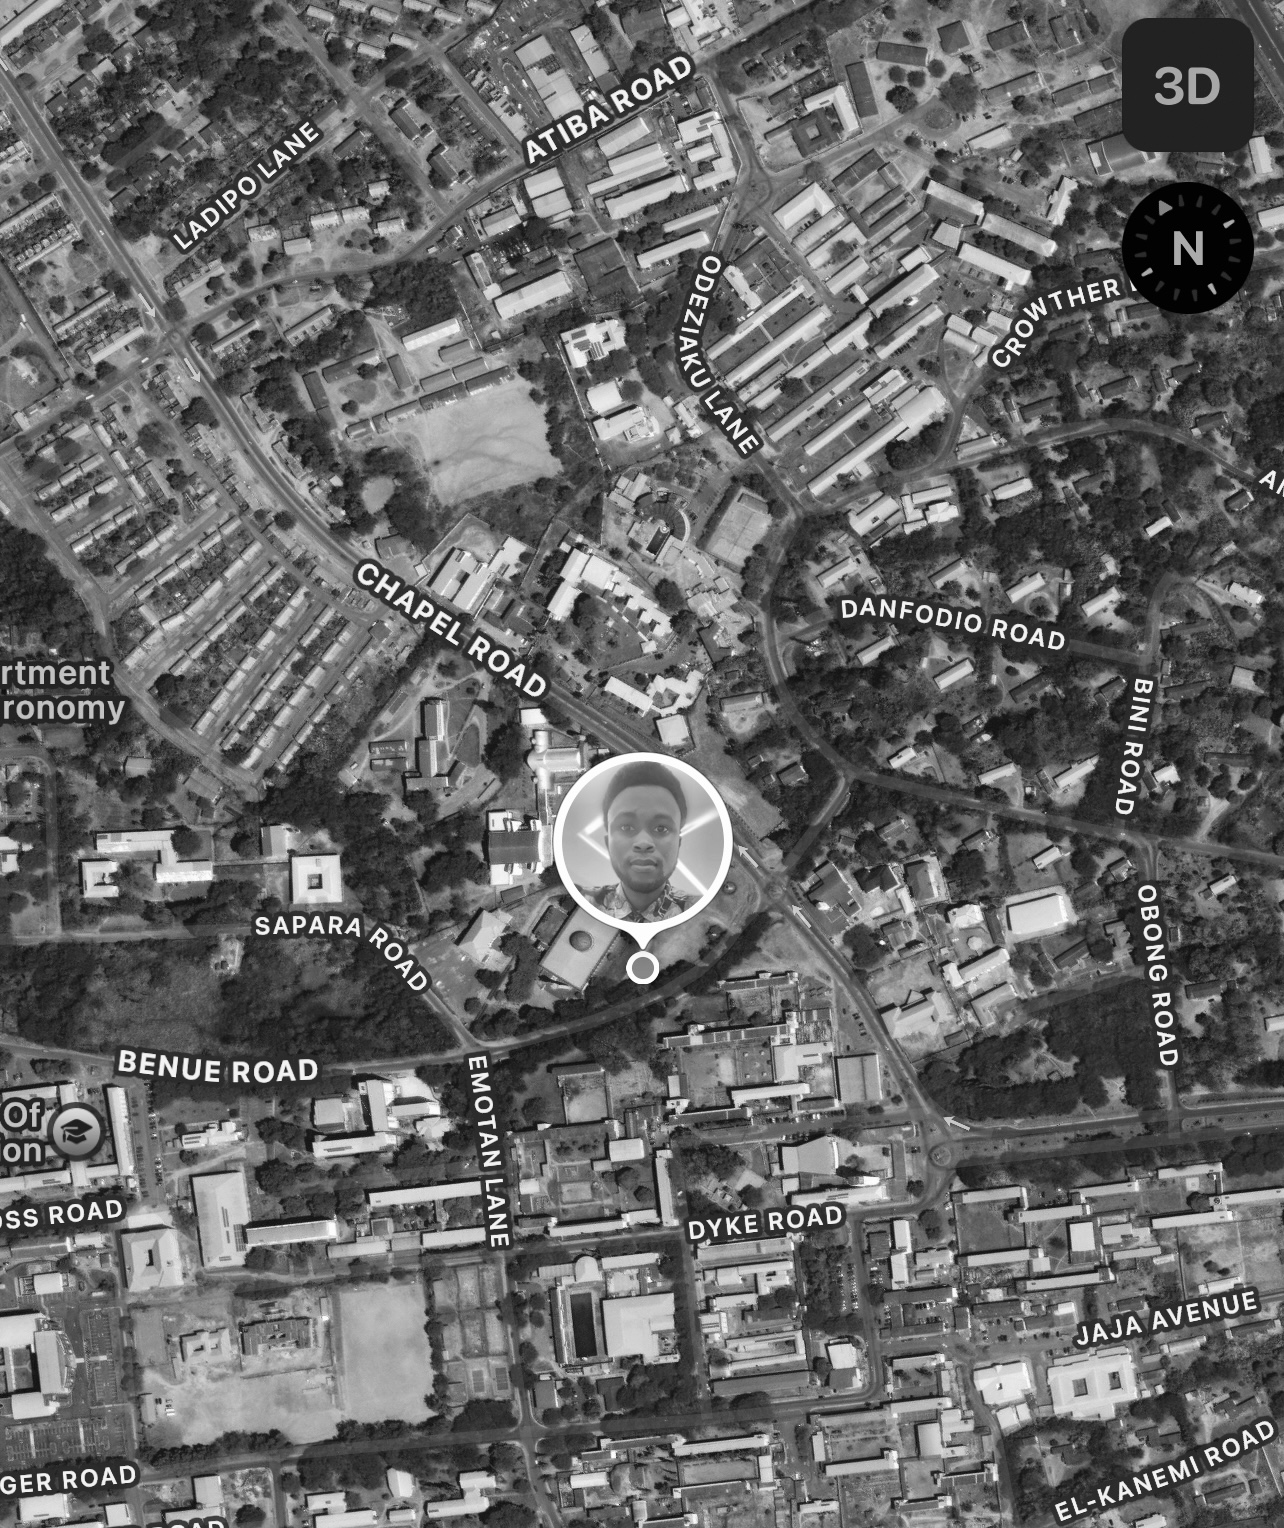
\includegraphics[width=1.0\textwidth]{AAHMap.jpg}
        \caption{\textbf{Coordinates:} 7.43933° N, 3.89449° E.}
        \label{fig:second}
\end{figure}

\newpage
\section{Outline of the Thesis}
This thesis is organized into five chapters:
\begin{itemize}
    \item Chapter 1: Introduction, including the aims, objectives, the study location and area including the significance of the study.
    \item Chapter 2: Literature Review, providing a detailed discussion of previous research, theoretical principles, applications, challenges and the limitations of the study.
    \item Chapter 3: Materials and Methods of the research and analysis.
    \item Chapter 4: The results, analysis, combination of VES and CST and further discusion.
    \item Chapter 5: Summary, Conclusion and Recommendations
\end{itemize}
References were also included at the end of the project

% Chapter 2: LITERATURE REVIEW
\chapter{CHAPTER 2: LITERATURE REVIEW}
\numberwithin{equation}{chapter}

\section{Introduction to Geophysical Methods in Civil Engineering}
Geophysical methods are generally non-invasive or non destructive methods long used in the construction industry for investigation of the subsurface. Principally, these are used for the detection of geologic anomalies such as cavities and voids, detection of buried pipes and other utilities, detection of water bearing aquifers for well development, exploitation of quarries and in determining soil stratification or layering. In addition, the methods provide a means for verifying as constructed pavement thicknesses in a continuous unbroken image of the pavement structural configuration or determining rebar embedment and layout non destructively.

The use of Geophysical methods confers advantages as they generally speed up the process of investigation, provide continuous streams of information not otherwise available in discrete sampling or invasive procedures and give advance information on what to expect for a given locality before a more detailed and costly soil exploration is even planned. Thus Geophysical methods are a force multiplier for the engineer and allow the user to identify potential problem areas or target areas even before the start of a detailed Soil Exploration program.

Geophysical methods are not a replacement to a detailed soil exploration program; rather they augment these programs to yield more meaningful and area extensive but more intensive information at the fraction of the time and cost. Geophysical Methods have been around for quite some time. These are non invasive procedures employed in order to determine subsurface soil conditions and geologic anomalies such as cavities and voids or buried objects such as pipelines. Geophysical methods are used for various purposes in Civil Engineering Investigation of the subsurface. The advent of high speed computers and fast signal processors have vastly improved the technology and resulted in increased reliability and signal clarity in the use of these methods.

\textbf{Emilio M. Morales \textit{et al.,}} in their Paper titled \textbf{\textit{Geophysical Methods in Civil Engineering – Practical Applications}} presented their local practical experience in the deployment of Geophysical methods and equipment to address and provide solutions to various practical problems where conventional approaches may not give adequate information or may not provide it in a faster or more accurate way. Although Geophysical methods address the need for more information compared to conventional borings, these are not substitute to actual soil borings particularly when soil design parameters (strength and compressibility) are needed. However, borings may provide only limited discrete information points or are limited because of budgetary restrictions while Geophysical methods may provide a continuous data stream or even three dimensional images of the desired target of interest. Thus these two methods are complementary and would provide a more meaningful information record when done together or when augmented by each other.

Although again these methods are not a substitute for detailed borings except for specific objectives which do not require strength characterization or design strength or compressibility parameters, they can sometimes yield more meaningful results and thus corroborate results of other methods.

\section{Overview of Geophysical Techniques}
Geophysical techniques offer innovative, non-invasive solutions for subsurface investigations, which are crucial in civil engineering projects. These methods provide reliable data on subsurface conditions, enabling engineers to make informed decisions regarding foundation designs, groundwater exploration, and the detection of subsurface anomalies. Among the most prominent techniques are \textbf{Ground Penetrating Radar (GPR)}, \textbf{Seismic Refraction}, and \textbf{Electrical Resistivity Methods}, each with unique principles, applications, and limitations.

\subsection{Ground Penetrating Radar (GPR)}
Ground Penetrating Radar (GPR) is a geophysical method that uses electromagnetic radar pulses to investigate the subsurface. Initially developed for military applications, such as detecting mines and buried weapons, GPR has become an essential tool in civil engineering due to its ability to provide high-resolution, real-time subsurface imaging.

\subsubsection{Principle of Ground Penetrating Radar}
GPR operates by transmitting electromagnetic radar impulses into the ground. The radar waves are reflected or absorbed based on the material's stiffness, moisture content, and composition. Reflected signals are captured by a receiving antenna and processed in real time to produce a subsurface image. The depth of investigation is inversely proportional to the radar frequency: higher frequencies provide better resolution at shallow depths, while lower frequencies are used for deeper penetration.

\subsubsection{Applications of Ground Penetrating Radar}
In a highway construction project, GPR is used to measure pavement thickness to millimeter precision, enabling dispute resolution and ensuring compliance with quality standards. GPR is versatile, with applications including:
\begin{itemize}
    \item Detection of cavities, voids, and geologic anomalies.
    \item Locating buried objects, such as pipelines, rebar, and archaeological artifacts.
    \item Environmental scanning for waste landfill detection.
    \item Measuring roadway and pavement thickness for quality assurance.
    \item Structural assessment of concrete to detect embedded objects.
\end{itemize}

\begin{figure}[h]
    \centering
    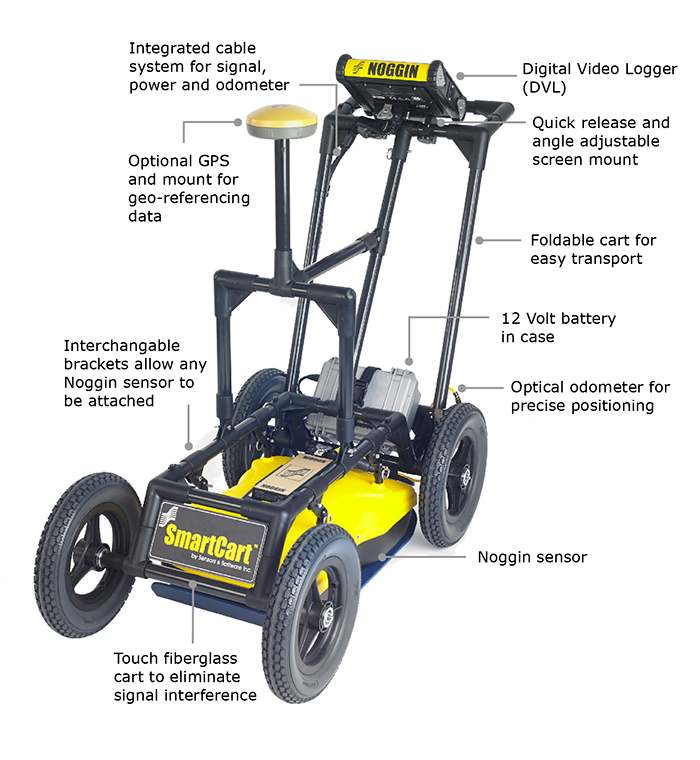
\includegraphics[width=0.5\textwidth]{GPR_img2.jpg}
    \caption{Diagram of well labeled GPR Equipment.}
\end{figure}

\subsubsection{Inherent Limitations of Ground Penetrating Radar}
\begin{itemize}
    \item Signal attenuation in conductive soils, such as clay, reduces penetration depth.
    \item The method's resolution decreases with increasing depth.
    \item Interpretation requires expertise and can be affected by noise and interference.
\end{itemize}

\subsection{Seismic Refraction Methods}
In a slope stabilization project, seismic refraction identified fault zones and sloping bedrock, enabling engineers to optimize foundation placement and reduce risks of structural failure. Seismic refraction is a method that utilizes shock waves to analyze subsurface structures and material properties. It is particularly effective for investigating stratigraphy and mechanical properties of soils and rocks.

\subsubsection{Principle of Seismic Refraction Methods}
Shock waves are generated by striking a steel plate with a hammer or using explosives. These waves travel through the ground, refracting and reflecting at material boundaries. Geophones positioned along a linear spread detect these waves, and their arrival times are recorded by a seismograph. The velocity of wave propagation provides insights into the stiffness and composition of subsurface layers.

\subsubsection{Applications of Seismic Refraction Methods}
\begin{itemize}
    \item Determining subsurface stratification and soil stiffness.
    \item Identifying faults, fractures, and cavities.
    \item Assessing sloping bedrock and geologic anomalies.
    \item Ensuring foundation stability in construction projects.
\end{itemize}

\subsubsection{Field Procedure of Seismic Refraction Methods}
A typical seismic refraction layout, known as a “spread,” involves 12 to 24 geophones. Multiple "shots" are conducted to ensure thorough coverage and accurate detection of subsurface anomalies. Each shot provides detailed data on layer characteristics and velocities.

\subsection{Electrical Resistivity Methods}
Surface electrical resistivity surveying is based on the principle that the distribution of electrical potential in the ground around a current-carrying electrode depends on the electrical resistivities and distribution of the surrounding soils and rocks.  The usual practice in the field is to apply an electrical direct current (DC) between two electrodes implanted in the ground and to measure the difference of potential between two additional electrodes that do not carry current.  Usually, the potential electrodes are in line between the current electrodes, but in principle, they can be located anywhere.  The current used is either direct current, commutated direct current (i.e., a square-wave alternating current), or AC of low frequency (typically about 20 Hz).  All analysis and interpretation are done on the basis of direct currents.  The distribution of potential can be related theoretically to ground resistivities and their distribution for some simple cases, notably, the case of a horizontally stratified ground and the case of homogeneous masses separated by vertical planes (e.g., a vertical fault with a large throw or a vertical dike).  For other kinds of resistivity distributions, interpretation is usually done by qualitative comparison of observed response with that of idealized hypothetical models or on the basis of empirical methods.

Mineral grains comprised of soils and rocks are essentially nonconductive, except in some exotic materials such as metallic ores, so the resistivity of soils and rocks is governed primarily by the amount of pore water, its resistivity, and the arrangement of the pores.  To the extent that differences of lithology are accompanied by differences of resistivity, resistivity surveys can be useful in detecting bodies of anomalous materials or in estimating the depths of bedrock surfaces.  In coarse, granular soils, the groundwater surface is generally marked by an abrupt change in water saturation and thus by a change of resistivity.  In fine-grained soils, however, there may be no such resistivity change coinciding with a piezometric surface.  Generally, since the resistivity of a soil or rock is controlled primarily by the pore water conditions, there are wide ranges in resistivity for any particular soil or rock type, and resistivity values cannot be directly interpreted in terms of soil type or lithology.  Commonly, however, zones of distinctive resistivity can be associated with specific soil or rock units on the basis of local field or drill hole information, and resistivity surveys can be used profitably to extend field investigations into areas with very limited or nonexistent data.  Also, resistivity surveys may be used as a reconnaissance method, to detect anomalies that can be further investigated by complementary geophysical methods and/or drill holes.

The electrical resistivity method has some inherent limitations that affect the resolution and accuracy that may be expected from it.  Like all methods using measurements of a potential field, the value of a measurement obtained at any location represents a weighted average of the effects produced over a large volume of material, with the nearby portions contributing most heavily.  This tends to produce smooth curves, which do not lend themselves to high resolution for interpretations.  Another feature common to all potential field geophysical methods is that a particular distribution of potential at the ground surface does not generally have a unique interpretation.  Although these limitations should be recognized, the non-uniqueness or ambiguity of the resistivity method is scarcely less than with the other geophysical methods.  For these reasons, it is always advisable to use several complementary geophysical methods in an integrated exploration program rather than relying on a single exploration method.

A single resistivity measurement requires four electrodes coupled to the ground and provides the apparent resistivity of the materials located between the potential electrodes. This surveys typically utilize multiple electrode pairs arranged in various configurations (i.e., spatial geometries), chosen based on site parameters and survey objectives \textbf{(Binley, 2015)}. In this project, I will discuss the two main approaches: \textbf{Vertical Electrical Sounding (VES)} and \textbf{Constant Separation Traversing (CST)} in detail later.

\section{Theoretical Background of Electrical Resistivity Methods}

\subsection{General Principles of Electrical Resistivity Methods}
The principle of electrical resistivity is based on Ohm's Law, which relates the flow of electric current through a material to its resistivity. Subsurface materials exhibit varying resistivity based on their composition, moisture content, and porosity. Conductive materials such as clays and water-saturated zones show low resistivity, while compact, dry rocks display high resistivity values. This variation allows for the characterization of subsurface layers.

\subsubsection{Principle of Resistivity}
Ohm's Law relates voltage ($V$), current ($I$), and resistance ($R$) through the equation:
\begin{equation}
    R = \frac{V}{I}
\end{equation}
In the context of subsurface investigations, resistivity ($\rho$) is calculated by considering the geometric dimensions of the material:
\begin{equation}
\rho = R \frac{A}{L}
\end{equation}

where:
\begin{itemize}
    \item $\rho$ = Resistivity of the material ($\Omega \cdot m$),
    \item $R$ = Measured resistance ($\Omega$),
    \item $A$ = Cross-sectional area of the material ($m^2$),
    \item $L$ = Length of the material ($m$).
\end{itemize}

\begin{figure}[h]
    \centering
    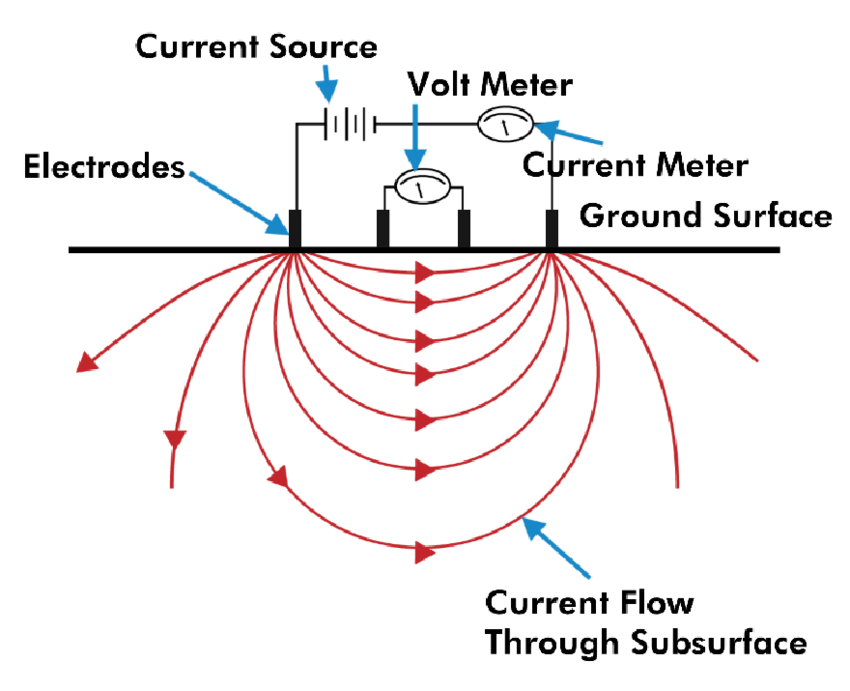
\includegraphics[width=0.75\textwidth]{current-flow.png}
    \caption{Diagram illustrating electrical current flow through subsurface}
\end{figure}

\subsubsection{Key Concept:}  
Conductive materials like clays and water-saturated zones have low resistivity, while dry, compact rocks and non-porous materials exhibit high resistivity. This contrast enables the detection of geological features such as aquifers, fractures, and stratigraphic boundaries.

\subsection{Electric Current Flow in Subsurface Materials}
When an electric current is introduced into the subsurface, it spreads radially through the soil or rock. The current's behavior depends on the material's resistivity, with high-resistivity materials offering greater resistance to current flow and low-resistivity materials allowing easier passage. The electric field generated by the current is measured using potential electrodes.

\subsubsection{Equation for Current Density:}
\begin{equation}
J = \sigma E
\end{equation}
where:
\begin{itemize}
    \item $J$ = Current density ($A/m^2$),
    \item $\sigma$ = Electrical conductivity ($1/\rho$, $S/m$),
    \item $E$ = Electric field intensity ($V/m$).
\end{itemize}

\subsection{Electrical Field and Potential}
When current is injected into the subsurface, it creates an electrical field. The potential difference ($\Delta V$) measured across two points is influenced by the resistivity of the intervening materials. Equipotential lines and current flow lines provide a visual representation of how the electrical field is distributed within the subsurface, aiding in the interpretation of resistivity data.

Coulomb established that the force of attraction or repulsion between two charged spheres is proportional to the product of the individual electric fields and inversely proportional to the square of the distance between the centers of the spheres. The electric field of a charge is a force \(\mathbf{F}\) exerted on another unit charge using Coulomb's law.

The force \(\mathbf{F}\) is given by:

\begin{equation}
\mathbf{F} \propto \frac{q_1 q_2}{r^2}
\end{equation}

Introducing the constant of proportionality \(k_e\), the equation becomes:

\begin{equation}
\mathbf{F} = k_e \frac{q_1 q_2}{r^2}
\end{equation}
\\
where:
\begin{itemize}
    \item \(\mathbf{F}\) is the force between the charges (in newtons, \(N\)),
    \item \(k_e\) is Coulomb's constant, approximately \(8.987 \times 10^9 \, \mathrm{N \cdot m^2 \cdot C^{-2}}\),
    \item \(q_1\) and \(q_2\) are the magnitudes of the charges (in coulombs, \(C\)),
    \item \(r\) is the distance between the charges (in meters, \(m\)).
\end{itemize}

The electric field (\(\mathbf{E}\)) at a point in space is defined as the force (\(\mathbf{F}\)) per unit charge (\(q\)):

\begin{equation}
\mathbf{E} = \frac{\mathbf{F}}{q} = k_e \frac{q}{r^2}
\end{equation}

This equation indicates that the electric field is radially outward for a positive charge and radially inward for a negative charge.

\subsubsection{Derivation of Electric Potential Formula}
Electric potential (\(V\)) at a point is defined as the work done in bringing a unit positive charge from infinity to that point in an electric field. The relationship between electric potential and the electric field is given by:

\begin{equation}
V = - \int \mathbf{E} \cdot d\mathbf{r}
\end{equation}

Substituting \(\mathbf{E} = k_e \frac{q}{r^2}\) into the equation:

\begin{equation}
V = - \int_{r_0}^{r} \left( k_e \frac{q}{r^2} \right) dr
\end{equation}

Evaluating the integral:

\begin{equation}
V = - k_e q \int_{r_0}^{r} \frac{1}{r^2} dr
\end{equation}

\begin{equation}
V = - k_e q \left[ -\frac{1}{r} \right]_{r_0}^{r}
\end{equation}

\begin{equation}
V = k_e q \left( \frac{1}{r_0} - \frac{1}{r} \right)
\end{equation}

For simplicity, when \(r_0 = \infty\), the potential at infinity is considered zero, and the equation becomes:

\begin{equation}
V = k_e \frac{q}{r}
\end{equation}

This equation shows that the electric potential at a distance \(r\) from a charge \(q\) is directly proportional to the charge and inversely proportional to the distance.

\subsubsection{Application to Resistivity Surveys}
In resistivity surveys, the potential difference (\(\Delta V\)) between two points on the subsurface is measured, and the apparent resistivity (\(\rho_a\)) is calculated. This potential difference is influenced by the distribution of current flow lines and equipotential surfaces, which vary based on subsurface resistivity.


\begin{figure}[h]
    \centering
    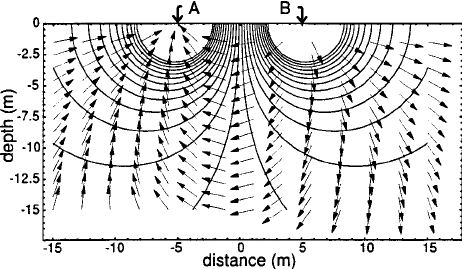
\includegraphics[width=0.8\textwidth]{ctf.png}
    \caption{Diagram illustrating electrical field with equipotential and current flow lines}
\end{figure}

\subsection{Apparent Resistivity}
Data from resistivity surveys are customarily presented and interpreted in the form of values of apparent resistivity \(\rho_a\). Apparent resistivity is defined as the resistivity of an electrically homogeneous and isotropic half-space that would yield the measured relationship between the applied current and the potential difference for a particular arrangement and spacing of electrodes. Wherever these measurements are made over a real heterogeneous earth, as distinguished from the fictitious homogeneous half-space, the symbol \(\rho\) is replaced by \(\rho_a\) for apparent resistivity.

Apparent resistivity is the bulk resistivity value obtained from field measurements. It is calculated using:
\begin{equation}
\rho_a = K \frac{\Delta V}{I}
\end{equation}

where:
\begin{itemize}
    \item $\rho_a$ = Apparent Resistivity ($\Omega m$),
    \item $\Delta V$ = Measured Potential Difference ($V$),
    \item $I$ = The Injected current ($A$).
\end{itemize}

Apparent resistivity is interpreted to estimate true resistivity, accounting for geological and geometric influences. Understanding apparent resistivity is crucial for interpreting field data and creating subsurface models.

\begin{figure}[h]
    \centering
    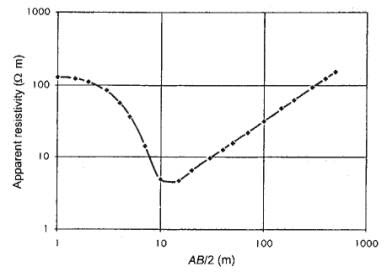
\includegraphics[width=0.75\textwidth]{apparent.jpg}
    \caption{Graph showing an apparent resistivity curve for a typical VES survey.}
\end{figure}

\section{Resistivity Surveying Techniques}

\subsection{Resistivity Surveying}
Resistivity surveying is a geophysical method used to explore and characterize the subsurface by measuring the electrical properties of the ground. This technique is particularly valuable for mapping various geological features such as stratigraphy, fractures, faults, and groundwater zones. By injecting electrical current into the ground and measuring the resulting potential differences, resistivity surveying provides insights into the distribution of materials with different electrical resistivities beneath the Earth's surface. These measurements are crucial for a variety of applications including environmental studies, engineering projects, archaeological investigations, and hydrogeological assessments.

The principle behind resistivity surveying is based on the fact that different materials, like clay, sand, rock, or water, have distinct electrical resistivities. For instance, water-saturated zones typically have lower resistivity due to the conductive nature of dissolved salts, whereas dry, compact rocks might show higher resistivity. By interpreting these resistivity variations, geophysicists can infer the presence of different subsurface layers or structures.

\subsubsection{Steps for carrying out Resistivity Surveying:}
\begin{enumerate}
    \item \textbf{Planning the Survey:} Before setting up, a detailed plan is created considering the survey objectives, the area's geology, and any known subsurface features. This includes choosing the appropriate electrode configuration (like Wenner, Schlumberger, or Dipole-Dipole arrays) based on the depth and resolution required.

    \item \textbf{Set Up Electrodes Along the Survey Line:} Electrodes are strategically placed along a predetermined line or grid pattern. The spacing between electrodes can vary depending on the desired resolution and depth of investigation. For deep surveys, wider spacing might be used, while for shallow investigations, closer spacing is preferred.

    \item \textbf{Inject Current Using an External Source:} An external power source, typically a battery or generator, is used to inject a known current into the ground through two current electrodes. The choice of current magnitude is important as it should be sufficient to produce measurable potential differences without causing electrode polarization or overheating.

    \item \textbf{Measure Potential Differences at Specific Electrode Configurations:} Using two potential electrodes, the voltage difference resulting from the current flow is measured. This step is repeated at various configurations or along the survey line to gather comprehensive data. Modern resistivity meters automate this process, ensuring precision in measurements.

    \item \textbf{Calculate Apparent Resistivity and Analyze Results:} The apparent resistivity is calculated using formulas that incorporate the measured potential difference, the injected current, and the geometric factor of the electrode array. This apparent resistivity might not directly represent the true resistivity due to the complex nature of subsurface materials but provides a basis for interpretation. 
    \begin{itemize}
        \item \textit{Data Processing:} Collected data is processed to remove noise, correct for any systematic errors, and sometimes to transform the data into a more interpretable form like 2D or 3D resistivity models.
        \item \textit{Interpretation:} Geophysical software or manual interpretation methods are used to analyze the resistivity data. This step involves correlating resistivity values with known geological properties, which might require integration with other geophysical or geological data.
        \item \textit{Validation:} Often, the results are validated through drilling or other direct methods to confirm the presence of predicted features like aquifers or fault lines.
    \end{itemize}
\end{enumerate}

\subsection{Vertical Electrical Sounding}
The vertical electrical sounding or geoelectric method is one of the most used electrical geophysical techniques thanks to its simplicity and relative low cost. These are especially useful in hydrogeological studies where it is necessary to define and characterize deep phreatic levels. Vertical electrical sounding or SEV are a geophysical technique that, by means of electricity, allows recognizing or distinguishing the different geological formations that are found in depth and delimiting them. Electrical or electromagnetic geophysical techniques are based on measuring the resistivity of materials or conductivity.

Vertical Electrical Sounding (VES) is a one-dimensional direct current electrical resistivity method, which consists of introducing a continuous electrical current of known intensity into the ground through two or more emitting electrodes, commonly called A and B, and measuring the electric potential difference using another pair of receiving electrodes, M and N, in this way it is possible to obtain the induced potential and the vertical distribution of the resistivities of the traversed formations. Using this method, the depth of study is directly proportional to the distance between the current electrodes and/or the potential electrodes used, so that the greater the separation distance between the electrodes, the greater the depth of the soil to be studied, while a spacing between the electrodes will measure the resistivity distribution in the subsurface at shallower depths. In this method, the results are compared with the common resistivities of the different materials, which allows them to be differentiated from each other.

The current injection electrodes A and B, and the potential measurement electrodes M and N, are arranged aligned in a certain structure, for this different configurations called “electrode device” are used, some of the most used are the Schlumberger configuration , Wenner and Dipole-Dipole.

\subsection{Constant Separation Traversing}
The object of electric horizontal profiling or combined Traversing
approach is to detect the lateral variations in the resistivity of the ground. In
Schlumberger method of electrical profiling, the current electrodes (AB)
remains fixed at a relatively large distance, for instance, a few hundred meters,
and the potential electrodes (MN) with a small constant separation (Sharma ,
1986).

The appearance of the resistivity profile obtained by horizontal profiling will
depend not only on the positions of the potential electrodes M and N, but also
on the positions of the current electrodes A and B with respect to the
inhomogeneities in the earth and the reason behind that is that all electrodes are
moved after each measurement (Kunetz, 1966).

The effect of vertical structures e.g. (faults, fissures, dikes, veins, and shear
zones) is lateral. If these features crop out, abrupt discontinuities in the slope of
\((\rho_a\)) curves are obtained as the mobile electrode configuration crosses the
vertical resistivity boundary. Many of key features found in the resistivity
anomalies over a vertical fault are found also in anomalies over near vertical
structures. The fault represents a vertical contact problem between two media of
differing resistivity. Therefore, the calculated curves for \((\rho_a\)) are discontinuous
at the vertical boundary. The discontinuity will be evident in practice as a steep
gradient in the resistivity curve (Sharma, 1986).

The traversing obtained by moving an electrode spread with fixed electrode
separation along a traverse line, the array of electrodes being aligned either in
the direction of the traverse (longitudinal traverse) or at right angles to it
(transverse traverse). The former technique is more efficient as only a single
electrode has to be moved from one end of the spread to the other, and the
electrodes reconnected, between adjacent readings. The Vertical discontinuity
distorts the direction of current flow and thus the overall distribution of
potential in its vicinity. (VES) data from several soundings can be presented in
the form of a pseudosections and it is now possible to invert the data into a full,
two-dimensional geoelectric model rather than a sequence of discrete, unidimensional geoelectric sections. This technique is known as electrical imaging
or electrical tomography (Kearey et.al, 2002).

\subsection{Comparison of VES and CST}


\begin{tabular}{|>{\raggedright\arraybackslash}m{4cm}|>{\raggedright\arraybackslash}m{6cm}|>{\raggedright\arraybackslash}m{6cm}|}
    \hline
    \textbf{Aspect} & \textbf{VES (Vertical Electrical Sounding)} & \textbf{CST (Constant Separation Traversing)} \\ \hline
    
    \textbf{Application} & Used for determining vertical variations in subsurface resistivity, often for geological or hydrological studies. & Used for mapping horizontal variations in subsurface resistivity over a specific area. \\ \hline
    
    \textbf{Field Survey} & Involves inserting electrodes into the ground at different depths along a vertical profile to measure resistivity changes with depth. & Electrodes are placed at a constant separation, and measurements are taken as the array is moved horizontally across the survey area. \\ \hline
    
    \textbf{Cost} & Costs include equipment, labor for setting up electrodes at various depths, and data analysis. & Similar costs but potentially less labor-intensive as electrode setup is simpler with fixed separation. \\ \hline
    
    \textbf{Formula} & Resistivity is calculated using formulas like $\rho_a = \pi a \left[ \frac{s^2}{a} - \frac{a}{4} \right] \frac{V}{I}$ \cite{web:0}. & Similar resistivity formulas but applied in a horizontal context, often using a Wenner or Schlumberger array configuration. \\ \hline
    
    \textbf{Purpose} & To provide a vertical profile of resistivity, useful for identifying depth to bedrock, water table, or different soil layers. & To provide a horizontal map of resistivity, useful for detecting lateral changes like faults, buried structures, or contaminant plumes. \\ \hline
    
    \textbf{Advantages} & Offers detailed information on vertical resistivity changes, which can be critical for depth-specific investigations. & Efficient for covering large areas to identify lateral resistivity variations, providing a broader spatial understanding. \\ \hline
    
    \textbf{Challenges} & Requires precise depth control and can be influenced by surface conditions; time-consuming for deep profiling. & Less detailed in vertical resolution, and lateral resolution depends on electrode spacing; can be affected by surface irregularities. \\ \hline  
\end{tabular}

\subsection{The General Four Electrode System}
The four-electrode system is a standard configuration for resistivity surveys, comprising two current electrodes (A and B) and two potential electrodes (M and N). This setup minimizes contact resistance effects and ensures accurate measurements. The purpose is to measure the electrical resistivity of materials or earth layers by eliminating contact resistance between the electrodes and the material.

\subsection{Electrode Configuration}
Electrode configuration (electrode array) A geometrical pattern of electrodes used in electrical sounding, constant-separation traversing, and induced polarization surveys. Usual configurations comprise two current electrodes and two potential electrodes whose separations are known and defined by a geometric factor. Common configurations include the Schlumberger arrays, Wenner arrays and dipole-dipole.

\subsubsection{Schlumberger Array:} 
Ideal for vertical profiling and depth estimation and commonly used in \textbf{Vertical Electrical Sounding (VES)} Surveying For this array, in the limit as \textit{a} approaches zero, the quantity V/a approaches the value of the potential gradient at the midpoint of the array.  In practice, the sensitivity of the instruments limits the ratio of s to a and usually keeps it within the limits of about 3 to 30.  Therefore, it is typical practice to use a finite electrode spacing. The apparent resistivity (r) is:

\begin{equation}
    \rho_a = \pi a \left[ \frac{s^2}{a} - \frac{a}{4} \right] \frac{V}{I} = \pi a \left[ \left( \frac{s}{a} \right)^2 - \frac{1}{4} \right] \frac{V}{I},
\end{equation}

\subsubsection{Wenner Array:}
This is suitable for horizontal profiling with uniform sensitivity and commonly used in \textbf{Constant Separation Traversing (CST)} Surveying. This array consists of four electrodes in line, separated by equal intervals, denoted a. After derivation, the user will find that the geometric factor K is equal to a , so the apparent resistivity is given by:

\begin{equation}
    \rho_a = \pi a \left[ \frac{s^2}{a} - \frac{a}{4} \right] \frac{V}{I} = \pi a \left[ \left( \frac{s}{a} \right)^2 - \frac{1}{4} \right] \frac{V}{I},
\end{equation}

\subsubsection{Dipole-Dipole Array:}
It provides high-resolution imaging for lateral changes. The dipole-dipole array is one member of a family of arrays using dipoles (closely spaced electrode pairs) to measure the curvature of the potential field.  If the separation between both pairs of electrodes is the same a, and the separation between the centers of the dipoles is restricted to a(n+1), the apparent resistivity is given by:

\begin{equation}
    \rho_a = \pi an (n + 1)(n + 2) \frac{V}{I},
\end{equation}
\\
\begin{figure}[h]
    \centering
    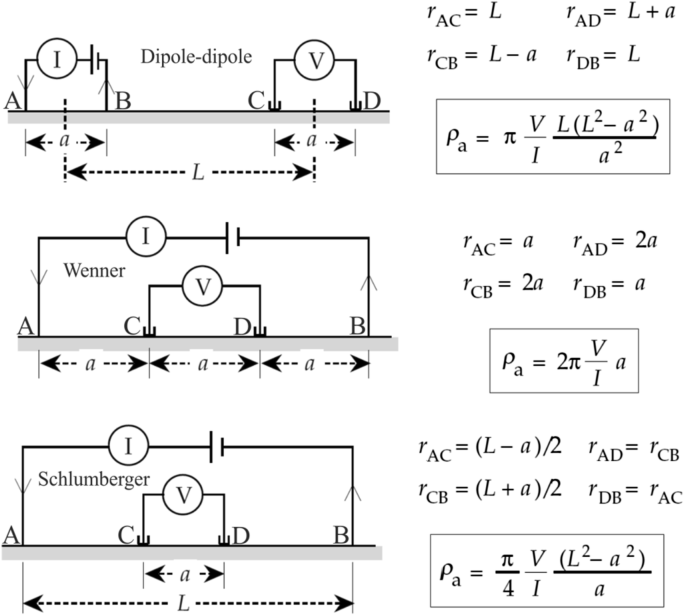
\includegraphics[width=1.0\textwidth]{wenschdip.png}
    \caption{Diagram illustrating current and potential electrodes for (a) Dipole-dipole (b) Wenner and (c) Schlumberger}
\end{figure}

\begin{figure}[p]
    \centering
    \begin{subfigure}[t]{0.9\textwidth}
        \centering
        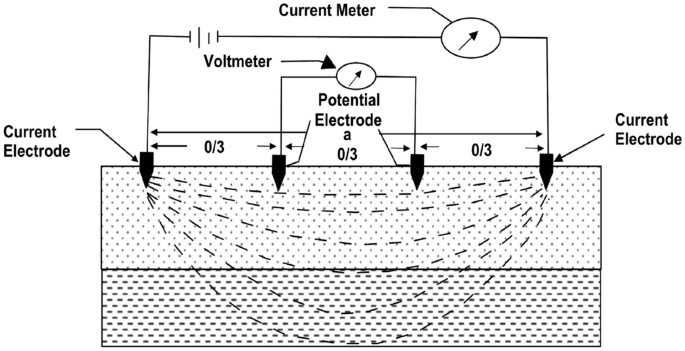
\includegraphics[height=0.3\textheight]{sclumberger.png}
        \caption{Schematic diagram of the Schlumberger array electrode configuration}
        \label{fig:schlumberger}
    \end{subfigure}\\[2cm]
    \vspace{1cm}
    \begin{subfigure}[t]{0.9\textwidth}
        \centering
        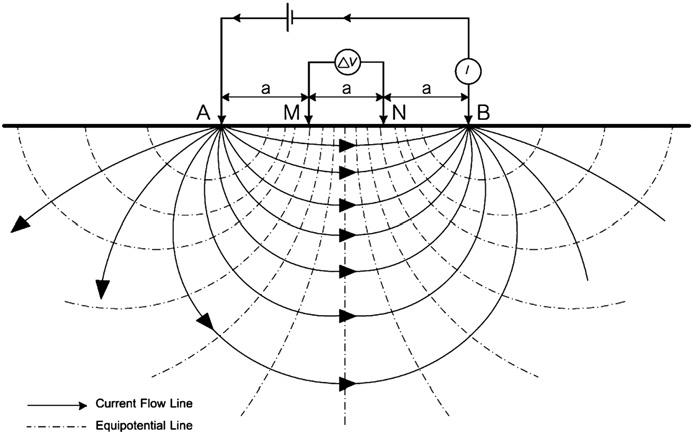
\includegraphics[height=0.35\textheight]{wenner.png}
        \caption{Schematic diagram of the Wenner array electrode configuration}
        \label{fig:wenner}
    \end{subfigure}
    \caption{Comparison of the Schlumberger and Wenner array electrode configurations.}
    \label{fig:configurations}
\end{figure}

\section{Previous Studies on Electrical Resistivity}

\subsection{Historical Context and Key Findings}
Electrical resistivity methods have evolved over the decades, with significant advancements in equipment and interpretation techniques. Early studies laid the groundwork for modern applications in groundwater exploration, mining, and foundation design. Previous studies have demonstrated the effectiveness of electrical resistivity in identifying subsurface anomalies such as fractures, cavities, and weak zones. These findings are crucial for designing safe and durable foundations.

\subsection{Previous Studies in Nigeria}

Several authors have contributed to the application of electrical resistivity methods in civil engineering investigations. Their works are summarized below:

\textbf{Akintoye et al. (2018)} investigated the subsurface conditions of an unstable slope in southwestern Nigeria using the electrical resistivity method. The study employed the Schlumberger configuration to delineate weak zones and fractures, revealing that high resistivity anomalies correspond to compact lithological units, while low resistivity zones indicate water-saturated regions. The results were used to recommend appropriate foundation designs for slope stabilization.

\textbf{Adeyemi and Bello (2020)} conducted a geophysical evaluation of construction sites in Lagos, Nigeria, to identify potential risks associated with heterogeneous subsurface layers. Using Vertical Electrical Sounding (VES), the authors mapped lithological variations and identified zones of high porosity and low bearing capacity. The findings highlighted the importance of resistivity surveys in mitigating structural failures.

\textbf{Olayemi et al. (2021)} applied electrical resistivity tomography (ERT) to assess subsurface integrity for a proposed bridge site. The study identified a highly fractured zone beneath the surface, which could pose a risk to structural stability. The authors recommended relocating the foundation to a more stable area, emphasizing the reliability of ERT in civil engineering applications.

\textbf{James and Olatunji (2019)} focused on the use of geophysics for groundwater exploration in arid regions. Though primarily aimed at water resource management, their work demonstrated the potential of resistivity methods in identifying zones with sufficient bearing capacity for construction purposes.

\subsection{Comparison of Methods}
Various configurations have been used in resistivity surveys, including Schlumberger, Wenner, and Dipole-Dipole arrays. \textbf{Eze et al. (2017)} compared these methods for subsurface investigations and found that the Schlumberger array is more effective for deep-layer detection, while the Wenner array provides better horizontal resolution. Their research underscores the need to select an appropriate configuration based on site-specific requirements.

\textbf{Telford et al. (1990)} further elaborated on the principles of resistivity methods, offering insights into how the Wenner array can be adapted for high-resolution near-surface investigations. Their book, \textit{Applied Geophysics}, is a seminal text that discusses various resistivity techniques and provides a detailed analysis of their applications in subsurface investigations. The authors emphasized that while the Schlumberger configuration excels in depth penetration, the Wenner method remains superior for detailed mapping of near-surface anomalies.

\textbf{Reynolds (2011)} provides a comprehensive guide on geophysical methods used in engineering, including electrical resistivity. In his book \textit{An Introduction to Applied and Environmental Geophysics}, he discusses how resistivity surveys are instrumental in civil engineering projects, especially in urban areas where the variability of subsurface properties poses significant challenges. He highlights the advantages of electrical resistivity tomography (ERT) for providing high-resolution images of the subsurface, which are crucial for detecting problematic zones in construction sites.

\section{Applications of Electrical Resistivity}

\subsection{Innovative Applications of Electrical Resistivity}
In recent years, there has been an increasing application of electrical resistivity methods in more complex subsurface investigations. \textbf{Steeples and Chilton (2001)} focused on the use of resistivity in mapping groundwater contamination in urban areas. They highlighted how advanced electrical resistivity tomography (ERT) can help locate pollution plumes in aquifers, enabling more efficient management of groundwater resources. Their work, published in \textit{Environmental and Engineering Geophysics}, underscores the growing versatility of resistivity methods in addressing both environmental and engineering concerns.

\textbf{Loke (2016)} provides a detailed exploration of the technological advancements in resistivity methods. In his book, \textit{Geoelectrical Imaging for Environmental and Engineering Applications}, he describes new developments in data acquisition systems, such as multi-electrode arrays, that have made resistivity surveys faster and more accurate. This book serves as a crucial resource for understanding the technical evolution of electrical resistivity methods and their broader application in modern engineering and environmental investigations.

\subsection{Applications in Structural Health Monitoring}
Electrical resistivity methods have also been explored for monitoring the health of structures over time. \textbf{Bermúdez et al., (2020)} demonstrated how electrical resistivity tomography can be employed to monitor the condition of reinforced concrete structures, detecting early signs of deterioration such as corrosion. Their study published in the \textit{Journal of Applied Geophysics} showed how resistivity surveys could be used for the non-destructive testing of infrastructure, offering a sustainable and cost-effective alternative to traditional inspection methods.

\textbf{Caldwell and Brown (2020)} conducted a study on the application of resistivity imaging for the monitoring of railway tracks. Their work showed that electrical resistivity could be used to detect subtle shifts in the ground around the tracks, which could indicate potential risks like landslides or subsidence. Their findings, published in the \textit{Geophysical Journal International}, suggest that resistivity surveys can play a critical role in maintaining the integrity of transport infrastructure, especially in areas prone to natural disasters.

\subsection{Applications in Building Foundation}
\textbf{Falae Philips Omowumi (2014)} carried out a geophysical survey using Vertical Electrical Sounding (VES) at Ibese Southwestern Nigeria in his book published in the \textit{Asia Pacific Journal of Energy and Environment, Volume 1, No 2 (2014)} to determine the geophysical parameters that can be used to evaluate the structural competence of the subsurface geological characteristics of the site for construction purposes and building development.

The Schlumberger configuration was used for the data acquisition. One-dimensional numerical inversion of individual DC resistivity was used to enhance the processing of the results for better achievement of the aim of the study. Models obtained from the 2D inversion of each VES were used for construction of geo-electric sections which exhibit the main geo-electric characteristics of the geological units present in thearea. 

\section{Importance of Subsurface Evaluation for Foundation Design}

Subsurface evaluation is a critical aspect of civil engineering, particularly in foundation design, as the stability, safety, and longevity of structures heavily depend on the underlying ground conditions. Inadequate knowledge of subsurface characteristics often leads to construction challenges, foundation failures, and increased project costs.

\subsection{Understanding Subsurface Conditions:}
The subsurface environment is inherently heterogeneous, comprising varying soil types, rock layers, and groundwater conditions. Evaluating these factors provides insights into:

\begin{itemize}
    \item \textbf{Soil Properties:} Characteristics such as density, cohesion, and angle of internal friction influence a soil's load-bearing capacity and compressibility.
    \item \textbf{Rock Layers:} The depth and quality of bedrock can affect the choice of foundation type and its depth.
    \item \textbf{Groundwater Table:} The presence of groundwater impacts soil strength and stability, making its identification crucial for waterproofing and structural integrity.
\end{itemize}

\subsection{Benefits of Subsurface Evaluation:}
\begin{itemize}
    \item \textbf{Foundation Stability:} Subsurface evaluation ensures that the chosen foundation type is compatible with site-specific conditions, reducing the risk of settlement or failure.
    \item \textbf{Cost Efficiency:} Early identification of subsurface issues prevents unforeseen complications during construction, minimizing delays and cost overruns.
    \item \textbf{Environmental Safety:} Identifying geological hazards such as faults, sinkholes, or contaminated soils mitigates risks to the structure and surrounding environment.
    \item \textbf{Design Optimization:} Provides engineers with critical data for designing efficient and durable foundations tailored to site-specific conditions.
\end{itemize}

\subsection{Geotechnical and Geophysical Contributions:}
Subsurface evaluations integrate geotechnical testing and geophysical methods to provide comprehensive insights. While geotechnical investigations offer detailed data on soil and rock mechanics, geophysical methods like electrical resistivity surveys, seismic refraction, and GPR complement these studies by mapping broader subsurface variations. Key contributions include:
\begin{itemize}
    \item Detecting weak zones or potential failure planes.
    \item Mapping soil stratigraphy and groundwater levels.
    \item Identifying the depth and properties of bedrock.
\end{itemize}

\subsection{Case Studies in Foundation Design:}
Several studies have demonstrated the importance of subsurface evaluation:
\begin{itemize}
    \item \textbf{Akintoye et al. (2018):} Used seismic refraction to detect weak zones in an unstable slope, enabling optimized foundation design for slope stabilization.
    \item \textbf{Adeyemi and Bello (2020):} Applied Vertical Electrical Sounding (VES) to map lithological variations in Lagos, Nigeria, identifying zones of low bearing capacity and mitigating risks of structural failure.
    \item \textbf{Olayemi et al. (2021):} Employed electrical resistivity tomography (ERT) to identify a fractured zone beneath a proposed bridge site, leading to the relocation of the foundation for safety.
\end{itemize}

\subsection{Relevance to Sustainable Construction:}
Subsurface evaluation aligns with sustainable construction practices by:
\begin{itemize}
    \item Minimizing material wastage through accurate design.
    \item Reducing the environmental impact of construction failures.
    \item Enhancing the resilience of structures against natural hazards.
\end{itemize}

\subsection{Conclusion:}
A thorough subsurface evaluation is indispensable in modern civil engineering. By combining geotechnical testing with advanced geophysical techniques, engineers can design safer, more efficient foundations that address the challenges posed by site-specific subsurface conditions. This integration not only ensures structural stability but also contributes to sustainable construction practices.

\chapter{CHAPTER 3: MATERIALS AND METHODS}

\section{Introduction}
This chapter outlines the materials, equipment, and methodologies employed in the geophysical evaluation of subsurface layers for civil engineering foundation design using electrical resistivity methods. The methods described here focus on Vertical Electrical Sounding (VES) and Constant Separation Traversing (CST), which were selected for their effectiveness in capturing vertical and lateral variations in subsurface resistivity. This chapter also discusses survey design, data acquisition, processing, interpretation, ethical considerations, and limitations encountered during the study.

\section{Geophysical Survey Materials and Equipment}
The success of a geophysical survey depends on the appropriate selection and utilization of specialized materials and equipment. The following tools were employed:

\begin{itemize}
    \item \textbf{Resistivity Meter:} The core device used to inject current into the ground and measure the resulting potential difference. A digital resistivity meter (e.g., ABEM Terrameter) was utilized for precise and reliable measurements.
    \item \textbf{Steel Metal Electrodes:} Used as current and potential electrodes for injecting current into the ground and measuring potential differences. Electrodes were securely inserted into the soil to ensure good contact.
    \item \textbf{Connecting Wire Cables:} Insulated cables connected the resistivity meter to the electrodes, ensuring stable current flow and accurate measurements.
    \item \textbf{Measuring Tape:} Used to measure and maintain accurate spacing between electrodes according to the selected configuration.
    \item \textbf{Hammer:} Assisted in driving electrodes into hard or compact ground surfaces.
    \item \textbf{Clips:} Metal clips were used to secure the cables to the electrodes and maintain strong connections.
    \item \textbf{Compass:} Used to align survey lines and ensure consistent electrode orientation relative to the site layout.
    \item \textbf{Global Positioning System (GPS):} Employed to accurately record the geographical coordinates of each survey station.
    \item \textbf{Data Recording Materials:} Included field notebooks, data sheets, and digital storage devices for logging measurements and observations.
\end{itemize}

\section{Methodology}

\subsection{Survey Design}

\begin{itemize}
    \item \textbf{Selection of Electrode Configurations:}  
    Two configurations were selected to address different investigation goals:
    \subsubsection{- Schlumberger Configuration:} This configuration was chosen for VES due to its ability to penetrate deeper into the subsurface by gradually increasing the current electrode spacing. It provides detailed depth-specific resistivity data and is cost-effective for deep investigations.
    \subsubsection{- Wenner Configuration:} This configuration was employed for CST as it is sensitive to lateral variations in resistivity, making it ideal for detecting horizontal changes in subsurface layers. Its simplicity in setup allows for rapid data acquisition over large areas.
    
    \begin{figure}[h]
        \centering
        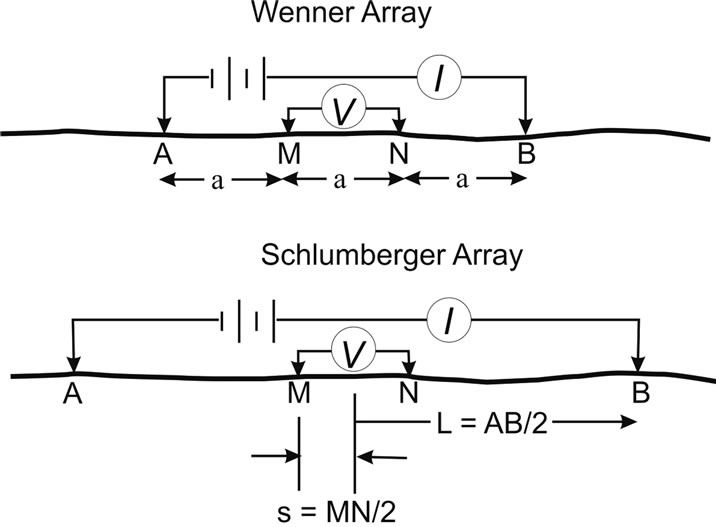
\includegraphics[width=0.75\textwidth]{wenner_schlum.jpg}
        \caption{Graph showing an apparent resistivity curve for a typical VES survey.}
    \end{figure}

    \item \textbf{Survey Layout:}  
    The study area was systematically covered using multiple parallel profiles spaced at regular intervals. Each profile's orientation was determined based on the geology and expected subsurface structures. The length and spacing of the profiles were optimized to balance survey resolution with field efficiency. GPS was used to mark electrode positions and ensure repeatability of the survey. \\ 
    \textbf{Image Suggestion:} Add a site map or grid layout showing the survey profiles and electrode placements within the study area.
\end{itemize}

\subsection{Field Procedures}
\begin{itemize}
    \item \textbf{Electrode Placement:} Electrodes were inserted into the ground at specified intervals based on the chosen configuration. Care was taken to ensure firm contact with the soil, especially in dry or compacted areas.
    \item \textbf{Current Injection and Measurement:} A steady electrical current was injected into the ground through the outer electrodes. The potential difference was measured across the inner electrodes using the resistivity meter. Environmental factors such as moisture levels and soil conductivity were monitored to optimize measurements.
\end{itemize}

\subsection{Data Acquisition}
\begin{enumerate}
    \item \subsubsection{Vertical Electrical Sounding Data Acquisition}
    Data was collected at fixed points along the survey line by gradually increasing the spacing between current electrodes. The resulting apparent resistivity values were plotted against electrode spacing to generate depth profiles.
    \item \subsubsection{Constant Separation Traversing Data Acquisition}
    The electrode array was moved laterally along the survey lines with a fixed electrode spacing. Apparent resistivity values were recorded at regular intervals to map horizontal variations in subsurface resistivity.
\end{enumerate}

\subsection{Data Processing}
\begin{itemize}
    \item \textbf{Software Used:} The data was processed using software such as RES2DINV and IPI2Win for 2D and 3D resistivity modeling. Surfer software was employed for contour plotting and visualization.
    \item \textbf{Data Correction:} Corrections were applied to remove noise caused by electrode polarization, environmental factors, or measurement errors. Calibration checks were performed to ensure the reliability of the resistivity meter.
    \item \textbf{Inversion Techniques:} The apparent resistivity values were inverted to obtain true resistivity, using iterative algorithms to refine the models. The final output included detailed resistivity profiles and maps.
\end{itemize}

\subsection{Interpretation Methods}
\begin{itemize}
    \item \textbf{Resistivity Models:} The processed data was used to construct 2D and 3D models of subsurface resistivity. These models highlighted lithological layers, groundwater zones, and potential weak zones.
    \item \textbf{Correlation with Geological Data:} Resistivity results were correlated with known geological features in the study area, including borehole logs and previous studies.
    \item \textbf{Validation:} Validation of the results was achieved by comparing the interpreted data with existing geological maps and, where available, borehole data.
\end{itemize}

\section{Limitations and Precautions}

\subsection{Limitations}
Electrical resistivity methods (ERM) are widely used for subsurface investigations, but they are not without limitations. These limitations can arise from environmental factors, methodological constraints, and inherent characteristics of the subsurface. Some of the key limitations include:

\begin{itemize}
    \item \textbf{Sensitivity to Noise:} ERM is highly sensitive to noise from external sources such as power lines, stray currents, and metallic objects in the survey area. These factors can distort measurements and affect data quality.
    \item \textbf{Limited Depth Penetration:} The depth of investigation is constrained by the maximum spacing of current electrodes. For deeper investigations, larger electrode spacing is required, which may not be feasible in restricted spaces or urban environments \textbf{(Binley, 2015)}.
    \item \textbf{Ambiguity in Interpretation:} Resistivity results are inherently non-unique, meaning that different subsurface conditions can produce similar resistivity patterns. This can lead to misinterpretation if additional validation methods, such as borehole logs, are not used \textbf{(Reynolds, 2011)}.
    \item \textbf{Effect of Geological Complexity:} In areas with highly heterogeneous geology, such as fractured zones or mixed lithologies, interpreting resistivity data can be challenging due to overlapping resistivity values \textbf{(Olayemi et al., 2021)}.
    \item \textbf{Dependence on Soil Moisture:} The resistivity of subsurface materials is strongly influenced by moisture content. Seasonal variations in soil moisture can lead to inconsistent results if surveys are conducted at different times of the year \textbf{(Farinde et al., 2015)}.
    \item \textbf{Environmental Impact:} In some cases, the insertion of electrodes can disturb the soil or vegetation. This is particularly a concern in sensitive ecological areas or agricultural lands.
    \item \textbf{Equipment Limitations:} The accuracy of resistivity measurements is dependent on the quality and calibration of the equipment used. Older or poorly maintained instruments can produce unreliable results.
    \item \textbf{Time and Labor Intensive:} Setting up electrodes and conducting surveys over large areas can be time-consuming, especially in rough terrains or areas with accessibility issues.
\end{itemize}

\subsection{Precautions}
To minimize the limitations of electrical resistivity methods and ensure reliable results, the following precautions should be taken:

\begin{enumerate}
    \item \textbf{Ensure Proper Electrode Contact:} Electrodes should be securely inserted into the ground to achieve good electrical contact. In dry or rocky areas, water or conductive gel can be used to improve contact.
    \item \textbf{Avoid Areas with High Noise Levels:} Surveys should be conducted away from power lines, pipelines, and other sources of electrical interference. If unavoidable, filters should be used to remove noise from the data.
    \item \textbf{Conduct Surveys During Stable Weather Conditions:} Avoid conducting surveys during extreme weather conditions, such as heavy rains or droughts, as these can affect soil resistivity and distort results.
    \item \textbf{Perform Regular Equipment Calibration:} The resistivity meter and other instruments should be calibrated before use to ensure accurate measurements. Regular maintenance is essential to avoid equipment malfunction.
    \item \textbf{Validate Results with Additional Methods:} To reduce ambiguity, resistivity results should be validated using borehole data, geological maps, or other geophysical methods like seismic or ground-penetrating radar (Reynolds, 2011).
    \item \textbf{Use Appropriate Electrode Configurations:} Select the electrode configuration (e.g., Schlumberger or Wenner) that best suits the survey objectives and site conditions. This ensures optimal resolution and depth coverage.
    \item \textbf{Minimize Environmental Impact:} Take measures to reduce soil and vegetation disturbance when placing electrodes, especially in environmentally sensitive areas.
    \item \textbf{Plan for Accessibility:} In areas with difficult terrain or limited access, plan the survey layout in advance to ensure all necessary locations can be reached without compromising data quality.
    \item \textbf{Conduct Pre-Survey Reconnaissance:} Assess the site for potential obstacles, such as rocks, buried utilities, or water bodies, that may interfere with the survey.
    \item \textbf{Record Detailed Field Notes:} Document all field conditions, instrument settings, and environmental factors during the survey. This information is crucial for data interpretation and troubleshooting.
\end{enumerate}

\chapter{CHAPTER 4: RESULTS AND ANALYSIS}
\end{document}
